% sage_latex_guidelines.tex V1.20, 14 January 2017

\documentclass[Afour,sagev,times]{sagej}
\usepackage{float}
\usepackage{array}
\usepackage{tabularx}
\usepackage{graphicx}
\usepackage{geometry}
\usepackage{longtable}
\usepackage{caption}
\usepackage{moreverb,url}

\usepackage[colorlinks,bookmarksopen,bookmarksnumbered,allcolors=black]{hyperref}

\newcommand\BibTeX{{\rmfamily B\kern-.05em \textsc{i\kern-.025em b}\kern-.08em
T\kern-.1667em\lower.7ex\hbox{E}\kern-.125emX}}

\def\volumeyear{2023}

\begin{document}

\runninghead{Völtzke}

\title{Sweet Dreams Ahead: Machine Learning Models for Nocturnal Hypoglycemia Prediction in Diabetes Type 2 Patients}

\author{Christoph Völtzke\affilnum{1}}

\affiliation{\affilnum{1}Utrecht University, Netherlands}

\corrauth{Christoph Völtzke, Utrecht University, Netherlands.}

\email{c.voltzke@stud.uu.nl}

\begin{abstract}
\textbf{Background and Aims:} Continuous glucose monitoring (CGM) is known to prevent adverse events such as nocturnal hypoglycemia (NH) in diabetes patients. However, due to its high cost, it is not feasible to provide CGM for the majority of Type 2 diabetes (T2D) patients, which implies a need for additional features to CGM that can help predict NH. While lifestyle factors such as diet and activity level are known to be related to T2D prevalence, the extent to which these factors can accurately predict NH has not yet been explored. To address this gap, this study developed predictive models for NH in T2D patients and compared the predictive performance of two feature conditions: one with CGM features included (Full data condition) and one without (Lifestyle condition).
\newline
\newline
\textbf{Methods:} Multiple machine learning (ML) algorithms were applied to data from 76 patients, where data is obtained from CGM, food diaries, physical activity trackers, and patient characteristics. Population models with multiple resampling and tuning strategies were trained with 10-fold cross-validation on a training set (75\%). The area under the receiver operating curve (AUC), Sensitivity (SENS), and Specificity (SPEC) were evaluated on a separate test set (25\%). For both data conditions, models across each ML algorithm were trained.
\newline
\newline
\textbf{Results:} In the Full data condition, a Random Forest (RF) model produced the best results(AUC=0.91, Se=0.89, Sp=0.83). In the Lifestyle condition, the best results were also achieved with an RF model (AUC=0.81, Se=0.81, Sp=0.71). Results were heterogeneous among the various machine learning algorithms and tuning strategies, indicating the need to compare multiple strategies.
\newline
\newline
\textbf{Conclusion:} Predictive performance is highest for models including CGM, however, in the absence of CGM the Lifestyle conditions indicated high AUC and SENS. These results demonstrated a cost- and time-effective way to identify T2D patients at risk.
\end{abstract}

\keywords{Decision-Support-System, Diabetes Type 2, Machine Learning, Nocturnal Hypoglycemia, Continous Glucose Measurement}

\maketitle

\section{Introduction}
\label{introduction}

Nearly 537 million adults worldwide are diagnosed with diabetes mellitus with a consistently rising prevalence \cite{federation2021idf}. Type 2 Diabetes (T2D) accounts for the clear majority with 90\% of all diabetes cases \cite{federation2021idf}. For T2D patients, medication, activity, and dietary habits are key elements in the management of keeping blood glucose levels within a regulated range to avoid adverse events. However, unregulated insulin treatment and unhealthy lifestyle habits may increase the risk of severe hypoglycemia leading to serious short-term consequences \cite{evans2013health}. In particular, nocturnal hypoglycemia (NH) is a common complication, with over 50\% of severe hypoglycaemic episodes occurring during night-time \cite{graveling2017risks}. NH can cause a range of symptoms like sleep disturbances, morning headaches, chronic fatigue, mood changes and is associated with cardiac arrhythmias, which can result in "death-in-bed syndrome" \cite{graveling2017risks}. In healthy subjects, hypoglycemia triggers awakening, however, diabetes patients are often unable to wake up when their blood glucose drops, showing the need for reliable prediction methods \cite{schultes2007defective}. 

A prominent approach is the integration of continuous glucose monitoring (CGM) into decision-support systems to assist diabetes patients with their self-management \cite{vettoretti2018continuous}. Decision-support systems enable a prediction at bedtime about the risk of adverse events, such as NH, and recommend measures to reduce complications \cite{cappon2017wearable}. Within these systems, machine learning (ML) models using CGM data have been successfully developed in Type 1 diabetes (T1D) patients to predict NH \cite{bertachi2020prediction,parcerisas2022machine,berikov2022machine,guemes2019predicting}. Despite accurate results in this population, research for T2D remains scarce. To the best of our knowledge, only a single study \cite{kronborg2022bedtime} predicts the risk of NH for T2D patients with a population limited to insulin-treated patients and CGM-based data. 

While CGM data is the most promising approach in predicting NH for T1D \cite{mujahid2021machine,felizardo2021data,zhang2023data}, its implementation on a large scale for T2D is not feasible due to high costs and monitoring frequency, leading to a higher risk of undetected NH episodes in T2D \cite{oyaguez2021cost,wood2018continuous}. As a result, additional features are needed such as physical activity and carbohydrate intake that are related to T2D prevalence and the occurrence of NH \cite{woodward2009nocturnal,wilson2015factors}. The use of lifestyle features instead of CGM features for NH prediction could reduce healthcare costs and help healthcare providers to develop further interventions. However, there is no information about the effectiveness of lifestyle features for NH prediction since most studies have focused on CGM features or combinations of multiple feature categories.

The limited availability of CGM data for T2D patients also impedes the most conventional approach of building personalized predictive models \cite{bertachi2020prediction,berikov2022machine,guemes2019predicting,mosquera2020predicting} for NH prediction. Personalized models require sufficient training data, spanning multiple days of tracking for each patient, which is generally the case for T1D patients as they are equipped with CGM in their daily life. However, typical CGM trackers for T2D patients have a short durability of 14 days \cite{oyaguez2021cost}, resulting in insufficient individual data sets for building accurate personalized models. As a result, alternative approaches such as population models are needed. Population models offer a cost and time-efficient way to assess the risk of NH by creating a common system for all users and utilizing baseline patient characteristics \cite{parcerisas2022machine}. To determine if population-based models are a viable alternative to personalized models it is important to investigate whether population models can accurately predict NH events in T2D.

Recent reviews \cite{mujahid2021machine,felizardo2021data,zhang2023data} further showed that the performance of different ML approaches varies with the study population, outcome definition, and training and validation approaches \cite{zhang2023data}. Especially, when investigating a new population, comparing and improving the predictive performance of multiple ML models and assessing their applicability in given clinical situations remains an important challenge.

Therefore, this study aims to address the challenges faced in NH prediction for a new population of T2D patients and to fill the gap in the literature, which has primarily focused on T1D patients. Specifically, this study investigates the use of lifestyle features, such as physical activity and carbohydrate intake, to predict, at bedtime, the risk of NH in T2D patients as an alternative to CGM data.

First, data processing, feature extraction, and feature selection have been applied. Second, multiple ML algorithms have been trained and optimized for two subsets of features with one including (Full data condition) and one excluding CGM (Lifestyle condition) to build population models. Third, the predictive performance between ML algorithms and also between the two data conditions have been compared. Last, the results have been critically evaluated to assess their impact on the existing literature and their contribution to the diabetes management of T2D patients.


\section{Method}
\label{Method}

\subsection{Databases}

Data for the present study originates from the “Diabetes and Lifestyle Cohort Twente” (DIALECT). DIALECT is an observational cohort study performed in the  Ziekenhuis Groep Twente (Netherlands) and is designed to investigate the effect of lifestyle and dietary habits as well as pharmacological treatment on outcomes in patients with T2D \cite{gant2017integrated}. The study included adult male and female patients with T2D (\textit{N=76}) who were monitored with a CGM system, a physical activity tracker, and kept dietary entries for up to 14 days, and only those with complete data on all three parameters for at least 5 days, along with baseline clinical patient information, were included in the analysis. Monitoring is conducted under free-living conditions at home. Blood glucose measurements every 15 minutes were recorded using the Abbott FreeStyle Libre as the CGM system, and after two weeks, the readers were returned, and the collected data were checked and uploaded. For physical activity tracking a non-invasive Fitbit wristband that measures every minute was used. During the two weeks of glucose measurements, patients were requested to maintain a food diary, which included details of the time, type, and quantity of food intake during those days.
This study was performed according to the declaration of Helsinki. Written informed consent was obtained from all patients before participation. The study has been approved by the local institutional review boards (FERB, Filed number: 22-1863) and is registered in the Netherlands Trial Register (NTR5855).

\subsection{Pre-Processing} \label{Pre-Processing}

For each patient the monitored days were divided into 24-hour periods, each of them starting at 6:00 am. This starting time is selected based on a visual inspection of the daily profiles and the average breakfast time. Daily profiles were further divided into day-time and night-time. Night-time was defined from 12:00 pm to 6:00 am to exclude the impact of the postprandial excursion after dinner and breakfast. For the feature extraction process, day-time is further divided into separate time intervals of 60 minutes from 4:00 pm until the pre-defined bedtime (12:00 pm) and an additional interval from 6:00 am to 4:00 pm. Daily profiles were excluded if multiple timestamps were missing in one of the time intervals during that 24-hour period. Further exclusion criteria are less than 50 steps completed and two or more missing timestamps for meals consumed in a single day, resulting in a total of \textit{N=713} daily profiles.

The occurrence of NH was defined when a patient spent at least a single measurement below 3.9 mmol/L (70 mg/dL), also known as level 1 hypoglycemia \cite{federation2021idf}, during night-time. The corresponding daily profiles were then labeled as nights with hypoglycemia and in all other cases as nights without hypoglycemia. 

\subsection{Feature extraction} \label{Feature extraction}
A total of 72 features were hand-crafted from CGM data, dietary entries, physical activity data, clinical patient information, and temporal-domain information. 

CGM-related features were extracted from each interval and for the full day-time. No features were included from CGM measures during night-time as the goal of this study was to predict the risk of NH in T2D patients before bedtime. First, descriptive statistics of the measured glucose concentrations were conducted for each interval and the full daytime. The assessed measures were the mean, standard deviation, minimum value, and maximum value. Further, occurrences of hyperglycemia- and hypoglycemia events over the day were extracted. Several indices of glucose variability and glycaemic control were assessed, which are commonly used in diabetology \cite{broll2021interpreting} including low- (LBGI) and high blood glucose index (HBGI), time in range, hyper- and hypoglycemia index, Glycaemic Risk Assessment Diabetes Equation (GRADE), and Glucose Management Indicator (GMI). All extracted indices have shown to be effective in predicting NH in diabetes patients \cite{sampath2016glycemic}. Further, three features were extracted based on slope coefficients from ordinary least square regressions with the purpose of gaining insights into the patterns and trends of glucose levels. Overall, this resulted in a total of 45 CGM-related features.

Next, 6 dietary features were extracted, including the sum of carbohydrate-, fat-, and calorie intake over the whole day. Past research showed that regarding food intake, the amount of carbohydrate intake has the strongest impact on the risk of NH \cite{hovorka2004nonlinear, bertachi2020prediction}. To account for the decreasing effect of carbohydrate intake on the blood glucose level a physiological model is applied. The carbohydrate onboard model (COB) \cite{hovorka2004nonlinear} was used on all meals ingested during the daytime, resulting in a single cumulative value representing the estimated remaining carbohydrates in plasma at bedtime. Last, the number of distinct meal times over the day is assessed as well as the time of the last meal before bedtime. 

Physical activity features include the total number of steps performed over the day and a feature obtained by applying the activity onboard model (AOB) \cite{oviedo2019minimizing}. This feature represents the accumulated effect of steps taken that day on the blood glucose level evaluated at bedtime. Dietary and physical activity features were defined as lifestyle features in this study and account for 8 features.

Several patient-related characteristics were extracted. These features were measurements at baseline including Hemoglobin A1c (HbA1c) values, patients' height, weight, sex, body mass index (BMI), age, and diabetes duration. Also, medical information like the type of medication (e.g. fast-acting insulin) and the doses prescribed were included as features, resulting in a total of 17 features.

Lastly, two temporal-domain features were included containing information about the day of the week and a distinction between weekends and work days. For a full description of all extracted features, see Supplementary Material \ref{tab:sup_1}.

\subsection{Feature Selection} \label{Feature Selection}
To select the most informative features for the model, a three-fold approach was employed including Mutual Information (MI) \cite{meyer2008information} criteria, Boruta feature selection \cite{kursa2010feature}, and expert knowledge.

MI is a model-independent method that captures non-linear relationships and interactions among features, thus, avoiding bias toward a particular model. MI quantifies the degree of dependence between two variables based on how much information they share, which for this study involves the comparison of their entropies. A threshold of 0.01 was applied to the MI values to identify features with meaningful associations with the target variable and avoid overfitting.

Boruta is a wrapper method incorporating an RF model. Boruta compares the importance of each feature with that of randomized shadow features to identify a relevant subset. Features with significantly higher importance based on mean decrease accuracy measure compared to their shadow features were considered relevant, while features with lower importance were considered irrelevant and removed in an iterative process. If the same variables were selected by both MI and Boruta, they were included in the final feature set as these features have been identified as important across both approaches.

The last step involved incorporating expert knowledge, where domain expertise and applicability of features in practice were considered. Furthermore, this step allowed for the inclusion of variables that may have demonstrated exceptional performance within one of the methods (MI or Boruta), but may not have met the threshold or importance criteria of the other method. 

By integrating these three steps, the feature selection process aimed to capture the most informative features for the predictive modeling task in a robust and unbiased manner, while also considering expert knowledge for interpretability and clinical relevance. 

This process is applied to the full data condition and also to the Lifestyle condition. For the full data condition, a feature space of 41 variables was selected and for the Lifestyle condition, 18 features were selected. The most important features based on the Boruta approach for each data condition are presented in Figure \ref{fig:features}.

\begin{figure}[tb]
\centering
\caption{Feature Importance values of 10 most important features for two conditions.}
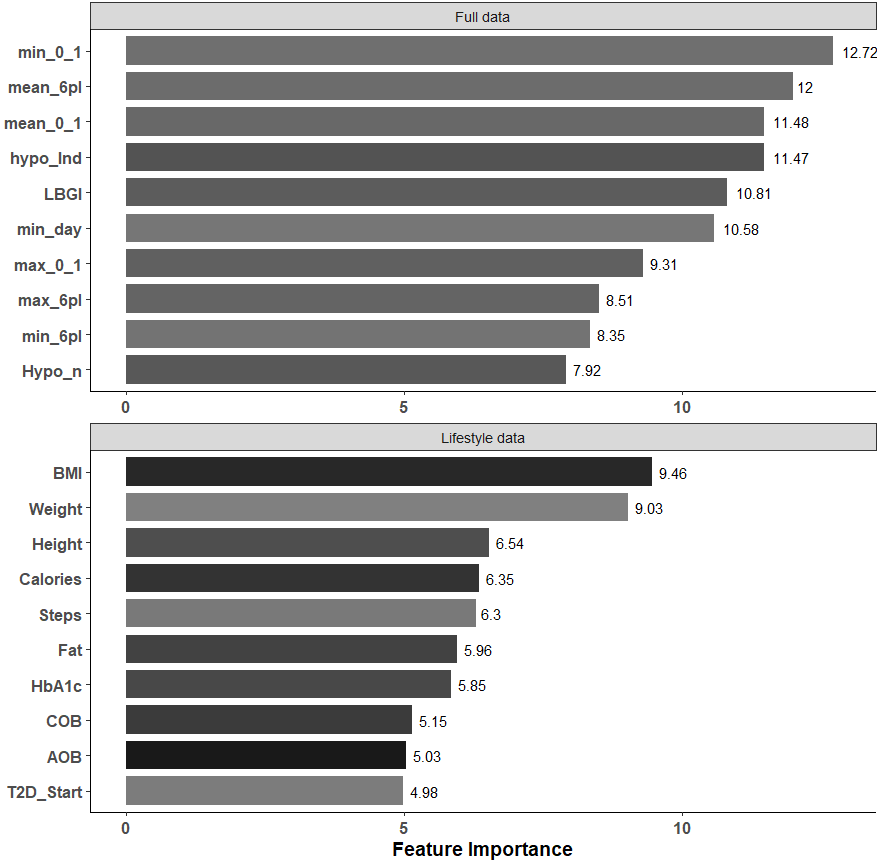
\includegraphics[width=0.5\textwidth]{Figures/Feature_Imp_rs.png}
  \parbox{0.45\textwidth}{\small{\textit{Note:} Abbreviations are explained in Supplementary Material \ref{tab:sup_1}. Feature Importance values are based on the mean decrease accuracy measure based on Boruta feature selection .}}
\label{fig:features}
\end{figure} 

\subsection{Machine Learning Algorithm Selection}  \label{Machine Learning Algorithm Selection}

To determine the best-performing model for the specific data characteristics, multiple ML algorithms were applied, including Random Forest (RF), Support Vector Machines (SVM), eXtreme Gradient Boosting (XGB), and Lasso logistic regression (Lasso). These algorithms were selected as they have been successfully used in previous studies for hypoglycemia prediction \cite{zhang2023data}.

RF is known for its ability to handle overfitting and has been used in multiple studies predicting hypoglycemia \cite{kodama2021ability,athey2019generalized}. SVMs are effective in high-dimensional datasets, can model nonlinear relationships between variables, and handle imbalanced data \cite{smola2004tutorial}. XGB is particularly successful in handling imbalanced data \cite{mujahid2021machine} and Lasso is useful for high-dimensional data as it performs another feature selection by shrinking the coefficients of less important features to zero \cite{kodama2021ability}.

The classifiers selected for this study were chosen for their ability to be integrated into decision support systems. All chosen ML algorithms have been shown to be accurate, transparent, interpretable, and computationally efficient, which makes them well-suited for practical applications \cite{mujahid2021machine, kodama2021ability}.

\subsection{Model Building Process} \label{Model Building Process}

\subsubsection{Model building preparation} \label{Feature category}
Class imbalance is a prevalent issue in the prediction of NH \cite{guemes2019predicting,parcerisas2022machine}, as observed in this study where only a small fraction of the recorded nights exhibited hypoglycemic events, leading to a bias towards the majority class. To address this issue, Up-sampling, Synthetic Minority Over-sampling Technique (SMOTE) \cite{chawla2002smote}, and cost-sensitive learning using threshold moving \cite{ling2008cost} were employed. Up-sampling involves replicating the minority class to balance the number of cases in each class. SMOTE generates synthetic samples of the minority class by interpolating between the minority class cases and their nearest neighbors, which has a lower risk of overfitting compared to Up-sampling. Both resampling strategies were employed on the training set only, as the test set should reflect the real-world distribution of the classes.

Cost-sensitive learning is applied to handle the varying costs of misclassification errors using threshold moving. The optimal threshold is chosen to be the point closest to the top-left part of the Receiver Operating Characteristic (ROC) curve with the highest sensitivity (SENS) or specificity (SPEC).
Within the threshold moving process, this study employed an increased weight to false negatives (FN), which refer to falsely classifying a night with hypoglycemia as a night without, compared to false positives (FP), which refer to falsely classifying a night without hypoglycemia as a night with. This weight was set to be twice the relative cost for an FN compared to an FP, which is in line with common clinical practice \cite{ling2008cost} as the cost of FN may lead to more consequences than the cost of FP.

Additionally, features are scaled to have a mean of zero and unit variance.

\subsubsection{Data split \& Cross-validation} \label{Data split}
The data was split into 25\% for testing and 75\% for training. To optimize the models' performance, 10-fold cross-validation was performed for the training set. This process was repeated for three folds of training data with different divisions of training and test data to overcome bias due to the small sample size. Mean and standard deviations (SD) over the three folds for the evaluation metrics were reported. Each ML algorithm was trained separately with different hyperparameter tuning strategies. Grid search with default values from the \texttt{caret} package \cite{kuhn2020package} for each ML classifier was used as a baseline, followed by a random search to broaden the search space of the hyperparameters. Additionally, a customized grid search was applied based on the best results of the first two searches and recommendations of search spaces from Probst et al.\cite{probst2019tunability}. Both SMOTE and Up-sampling techniques were applied during the cross-validation procedure to reduce bias in the sampling process. 

All tuning processes were applied to the original dataset, as well as to the up-sampled and SMOTE-generated datasets. The entire process, including data splitting, resampling, and model training, was repeated for both data conditions (Full data condition \& Lifestyle condition).

\subsection{Evaluating Model Performance} \label{Evaluating the Performance}
To evaluate the performance of the ML algorithms, widely-accepted evaluation metrics were used, such as SENS, SPEC, and AUC. 
    
\begin{center}
\begin{minipage}{0.25\textwidth}
\centering
\begin{equation}
\text{SENS} = \frac{\text{TP}}{\text{TP} + \text{FN}},
\label{eq:sens}
\end{equation}
\end{minipage}
\begin{minipage}{0.25\textwidth}
\centering
\begin{equation}
\text{SPEC} = \frac{\text{TN}}{\text{TN} + \text{FP}}.
\label{eq:spec}
\end{equation}
\end{minipage}
\end{center}

As shown in equation (\ref{eq:sens}), true positive (TP) represents that nights with hypoglycemia were correctly identified as hypoglycemic, and FN represents that nights with hypoglycemia were incorrectly identified as non-hypoglycemic. Therefore, SENS measures the proportion of positives (NH) that are correctly classified. In equation (\ref{eq:spec}), true negative (TN) represents that nights without hypoglycemia were correctly identified as non-hypoglycemic, and FP indicates that nights without hypoglycemia were incorrectly identified as hypoglycemic. Hence, SPEC shows the proportion of negatives (no NH) that are correctly identified.

Additionally, the AUC measures the ability of classifiers to distinguish between positive and negative cases across all possible classification thresholds. AUC is particularly useful when dealing with class imbalance as it is not affected by the threshold used to make predictions. Therefore, also not being affected by the applied cost-sensitive learning approach as it is independent of the threshold selection.

\subsection{Software} \label{Software}
Analyses and pre-processing are performed using \texttt{R version 4.2} \cite{team2020rstudio}. Model training and feature selection are conducted with the \texttt{caret} package. Class imbalance is handled with the \texttt{DMwR} package. Packages used for ML algorithms are \texttt{ranger} for RF, \texttt{kernlab} for SVM, \texttt{xgboost} for XGB, and \texttt{glmnet} for Lasso.
\section{Results}
\label{Results}

\subsection{Baseline \& Feature Selection results}
The baseline characteristics for the included patients are shown in Table \ref{tab:descriptives}. A total of 76 patients with 713 independent periods have been included. The prevalence of NH for these periods was 15.8 \% for the included patients. The average age was at 64.9 years (SD= 9.8) and the majority of patients were male (62.3 \%). The study population had a high average BMI of 30.5 (SD= 4.9).

Boruta feature selection and MI criteria identified the most important variables for the two data conditions. The Boruta approach revealed that in the full data condition, only two features (AOB and Diabetes duration) were included that were not extracted from CGM values. Further, CGM indices and descriptive statistics for the intervals of zero to one hour and over six hours before bedtime were considered the most important features. In the Lifestyle condition, features from all categories except temporal location were selected. The most important features were baseline patient characteristics, including BMI, height, and weight, followed by features from both lifestyle categories. The ten most important features based on Boruta for both conditions are shown in Figure \ref{fig:features}.
The results of the MI criteria mostly supported the decisions based on Boruta. Additionally, MI criteria identified several baseline characteristics (BMI, HbA1c values, weight, height, and age) that clearly shared information with the outcome variable. Within the lifestyle features, MI indicated that AOB, the sum of steps, and ingested calories shared most information with the outcome variable. Both feature selection methods suggested that medication- and temporal-location features were the least important for this predictive task.

\subsection{Model comparison}
In this study, the performance of 80 independent models using various ML algorithms, sampling and tuning strategies, and data conditions were evaluated. Specifically, four ML algorithms (RF, SVM, XGB, and Lasso) with three sampling strategies (Original, Smote, and Up-sampling), three tuning strategies (Default Grid, Random Grid, and Customized Grid), and two data conditions (Full data condition \& Lifestyle condition) were tested, resulting in a total of (4*3*3*2) 72 models. All of these models applied cost-sensitive learning by threshold moving. Additionally, for each combination of an ML algorithm and data condition (4*2), models with a threshold set to .5 for the prediction of the outcome, resulting in 8 additional models. This approach was repeated three times using different training and test data divisions, where means and SDs were conducted for each of the 80 models.

The best-performing tuning strategy, based on the model's average performance on the evaluation metrics, for each combination of an ML algorithm and sampling approach was selected, which resulted in a total of 32 models, presented in Table \ref{tab:results_all}. Across the selected models no superior tuning strategy could be identified.

The results showed that using sampling strategies to address the class imbalance, such as SMOTE and Up-Sampling, did not lead to better results compared to using the original data sampling. For the full data condition, the original sampling resulted in the best performance across all ML algorithms (AUC=0.88-0.91, SENS=0.85-0.89, SPEC=0.78-0.87). For the Lifestyle condition, no superior sampling strategy was identified for all evaluation metrics, but Up-Sampling showed less variability in its estimates compared to the original sampling. Although the difference between the three sampling methods was small in terms of AUC, it fluctuated more for both SENS and SPEC.

The findings further revealed that the cost-sensitive learning approach consistently resulted in higher SENS across all ML algorithms when compared to the models trained without cost-sensitive learning. Specifically, in the Lifestyle condition,  the difference in SENS is highest between the models that applied threshold moving compared to the no-cost models (SENS No-Cost=0.06-0.31, SENS Original=0.78-0.83).

Last, the results demonstrated that the choice of ML algorithm had only a minor impact on the evaluation metrics in the Full data condition, with RF (AUC=0.88-0.91, SENS=0.88-0.89, SPEC=0.75-0.83) achieving the best results, followed by XGB, SVM, and Lasso. In contrast, in the Lifestyle condition, while RF still performed the best, with XGB and SVM following closely, Lasso performed significantly worse in terms of AUC and SPEC. Specifically, Lasso achieved a much lower AUC (0.58) and lower SPEC (0.41-0.49) compared to other algorithms, although its SENS was still relatively high (0.73-0.80).

\newcommand*{\MyIndent}{\hspace*{0.5cm}}
\begin{table}[tb]
  \sf\centering
  \caption{Baseline Characteristics of Patients \textit{N = 76}.}
  \begin{tabular}{lcc}
    \hline
    \textbf{Variable} & \textbf{Mean (Proportion)}  & \textbf{SD (\%)} \\
    \hline
    
    Nocturnal Hypo. \\
       \MyIndent Yes & 113 & 15.8 \% \\   
       \vspace{0.15cm}
      \MyIndent No    & 600 & 84.2 \% \\
      \vspace{0.15cm}
    Age (years)& 64.9 & $\pm$ 9.8 \\
    Gender \\
       \MyIndent Female & 269 & 37.7 \% \\   
       \vspace{0.15cm}
      \MyIndent Male    & 444 & 62.3 \% \\
      \vspace{0.15cm}
    Height (cm) & 173.3 & $\pm$ 9.2 \\
    \vspace{0.15cm}
    Weight (kg) & 91.4 & $\pm$ 14.8 \\
    \vspace{0.15cm}
    BMI (kg/m^2) & 30.5 & $\pm$ 4.9 \\
    \vspace{0.15cm}
    HbA1c (mmol/mol) & 56.7 & $\pm$ 11.9 \\ 
    \vspace{0.15cm}
    Duration T2D (years) & 17.7 & $\pm$ 9.9 \\
    \hline
    \end{tabular} %
      \label{tab:descriptives}%
    \vspace{0.25cm}
  \parbox{0.45\textwidth}{\small{\textit{Note:} Continuous variables are presented by mean ± standard deviation and categorical variables by percentage (proportion).}}
\end{table}
  
\begin{table*} [tb]
\sf\centering
\caption{Averaged Performance Metrics and Standard Deviations for Model Comparison.}
\label{table:performance_metrics}
\begin{tabular}{cc|cccc|cccc}
\hline
\multicolumn{2}{c}{\textbf{}} & \multicolumn{4}{c}{\textbf{Full Data Condition}} & \multicolumn{4}{c}{\textbf{Lifestyle Condition}} \\ \cline{3-10} 
\textbf{Model} & \textbf{Metric} & \textbf{No-Cost} & \textbf{Original} & \textbf{SMOTE} & \textbf{Up} &  \textbf{No-Cost} & \textbf{Original} & \textbf{SMOTE} & \textbf{Up} \\ \hline
\multirow{\textbf{RF}} & \textbf{AUC}& 0.90 & \textbf{0.91} & 0.88 & 0.88 & 0.81 & 0.82 & 0.82 & 0.81 \\ 
& & (0.04) & \textbf{(0.03)} & (0.01) & (0.01) & (0.04) & (0.03) & (0.02) & (0.04) \\ 
 & \textbf{SENS} & 0.33 & \textbf{0.89} & 0.88 & 0.88 & 0.21 & 0.83 & 0.81 & 0.80 \\  
 & & (0.20) & \textbf{(0.08)} & (0.06) & (0.04) & (0.05) & (0.05) & (0.07) & (0.08) \\
 & \textbf{SPEC} & 0.97 & 0.83 & 0.78 & 0.75 & 0.97 & 0.69 & 0.71 & 0.72 \\ 
& & (0.03) & (0.05) & (0.05) & (0.01) & (0.02) & (0.07) & (0.06) & (0.04) \\  \hline
\multirow{\textbf{SVM}} & \textbf{AUC} & 0.89 & 0.89 & 0.86 & 0.88 & 0.78 & 0.78 & 0.78 & 0.78 \\  
& & (0.04) & (0.04) & (0.04) & (0.02) & (0.05) & (0.05) & (0.05) & (0.04) \\
 & \textbf{SENS} & 0.35 & 0.86 & 0.89 & 0.82 & 0.06 & 0.82 & 0.80 & 0.79 \\
& & (0.13) & (0.02) & (0.06) & (0.04) & (0.02) & (0.07) & (0.08) & (0.03) \\ 
 & \textbf{SPEC} & 0.97 & 0.87 & 0.70 & 0.84 & \textbf{1.00} & 0.60 & 0.67 & 0.66 \\   
& & (0.02) & (0.08) & (0.04) &( 0.02) & \textbf{(0.00)} & (0.05) & (0.10) & (0.07) \\  \hline
\multirow{\textbf{XGB}} & \textbf{AUC} & 0.89 & 0.90 & 0.89 & 0.90 & 0.81 & 0.81 & 0.79 & 0.78 \\  
& & (0.04) & (0.06) & (0.04) & (0.04) & (0.03) & (0.03) & (0.04) & (0.04) \\ 
 & \textbf{SENS} & 0.52 & 0.86 & \textbf{0.89} & 0.87 & 0.31 & 0.79 & 0.84 & 0.82 \\ 
& & (0.10) & (0.06) & \textbf{(0.03)} & (0.09) & (0.04) & (0.04) & (0.03) & (0.04) \\ 
 & \textbf{SPEC} & 0.95 & 0.82 & 0.78 & 0.81 & 0.97 & 0.74 & 0.62 & 0.64 \\ 
& & (0.03) & (0.06) & (0.07) & (0.06) & (0.00) & (0.04) & (0.03) & (0.05) \\ \hline
\multirow{\textbf{Lasso}} & \textbf{AUC}  & 0.88 & 0.88 & 0.85 & 0.86 & 0.58 & 0.58 & 0.58 & 0.58 \\ 
& & (0.06) & (0.05) & (0.07) & (0.05) & (0.05) & (0.06) & (0.03) & (0.06) \\ 
 & \textbf{SENS} & 0.38 & 0.85 & 0.83 & 0.82 & 0.22 & 0.78 & 0.80 & 0.73 \\  
& & (0.04) & (0.04) & (0.05) & (0.06) & (0.30) & (0.08) & (0.12) & (0.04) \\
 & \textbf{SPEC} & 0.96 & 0.78 & 0.74 & 0.76 & 0.81 & 0.45 & 0.41 & 0.49 \\ 
& & (0.01) & (0.06) & (0.14) & (0.05) & (0.17) & (0.03) & (0.10) & (0.04) \\ \hline
\end{tabular} %
\label{tab:results_all}%
 \vspace{0.25cm}
  \parbox{0.8\textwidth}{\small{\textit{Note:} The results are averaged over three folds and SDs are depicted within parentheses. Models are shown for 4 ML algorithms, with 3 distinct sampling strategies, and 2 data conditions. Models excluding cost-sensitive learning are shown in the columns "No Cost".  }}
\end{table*}%

\subsection{Difference between Lifestyle and CGM data}
This second part of the analysis focused on the comparison of the two data conditions. Only models using cost-sensitive learning were considered for comparison.

The results suggested that the inclusion of CGM features consistently resulted in higher AUC values compared to subsets without CGM, with AUC ranging from 0.85 to 0.91 for the Full data condition and 0.58 to 0.82 for the Lifestyle condition. In terms of SENS, the Full data condition ranged between 0.82 to 0.89, while the Lifestyle condition led to similar estimates, with SENS ranging from 0.73 to 0.84. In terms of SPEC, there was a consistently lower performance in the Lifestyle condition, with SPEC ranging from 0.41 to 0.74, compared to 0.70 to 0.87 for the Full data condition. The results of the ROC analysis for the two data conditions across the four ML algorithms and over the three folds are depicted in Figure \ref{fig:roc_curves}.

\begin{figure}[htbp]
\sf\centering
\caption{ROC curve comparison - Full Data Condition vs. Lifestyle Condition across all ML algorithms.}
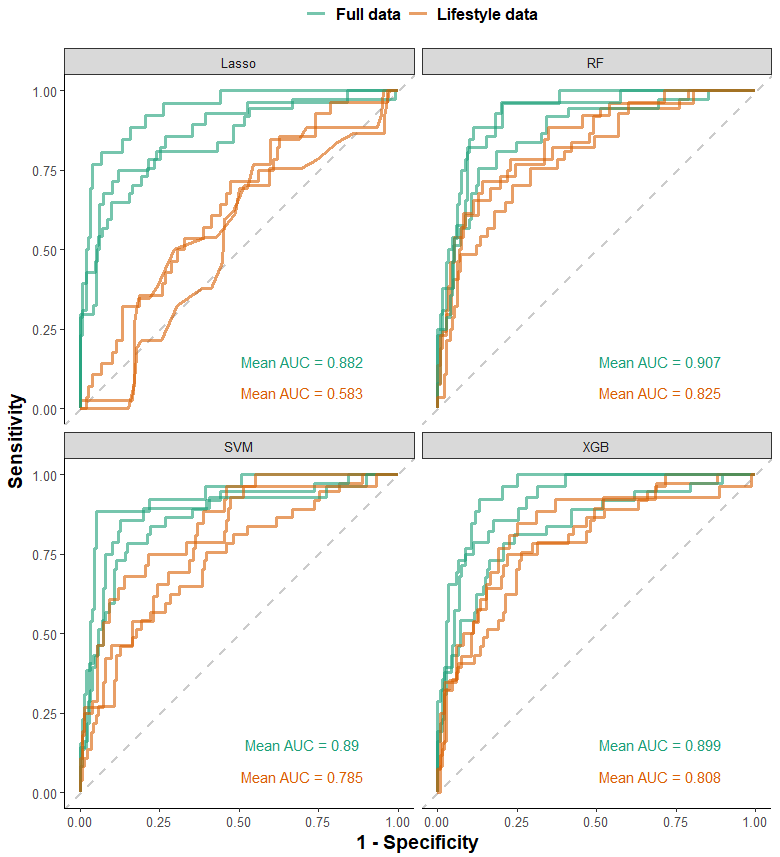
\includegraphics[width=0.5\textwidth]{Figures/ROC_compare_folds_rs.png}
\vspace{0.25cm}
  \parbox{0.45\textwidth}{\small{\textit{Note:} Same model building choices were applied across all three folds .}}
\label{fig:roc_curves}
\end{figure}
\section{Discussion}
\label{Discussion}

This study showed that ML-based prediction models can be successfully used to mitigate the risk of hypoglycemia in T2D patients. Furthermore, this study demonstrated that important contributions can be made toward hypoglycemia prevention in T2D by investigating models that excluded CGM data for model building.

This study contributes to the literature on predicting NH in T2D patients by incorporating a larger study population with more than double the sample size compared to a previous study. The study also includes a broader group of patients, including those without insulin treatment, and utilizes multiple data sources such as CGM, physical activity, dietary information, and patient characteristics. These findings enhance the generalizability of ML-based prediction models for T2D patients and further improve the development of preventative interventions.

To further assess the applicability in clinical situations various model-building decisions were tested in this study, which is specifically needed when dealing with unknown populations. The study included multiple ML algorithms, several tuning strategies, and distinct sampling approaches to compare and improve the predictive performance of the models. The results showed that the predictive performance varied across different ML algorithms, indicating the need to test multiple methods to see which approach fits best to the given data characteristics. For instance, the RF algorithm demonstrated superior performance in this study, indicating that it might be a suitable method for predicting NH in T2D patients. However, it is important to note that the performance of the ML algorithms depends on study characteristics, such as the study population, outcome definition, and validation approaches. Therefore, relying on a single ML algorithm may not be sufficient to achieve high predictive performance.

Additionally, in NH prediction, class imbalance is a common issue, and sampling approaches, such as SMOTE and Up-sampling, have been suggested to handle it. However, in this study, these techniques were found to have no advantageous impact on the model's performance, implying that other methods may be more effective. Specifically, cost-sensitive learning was found to significantly improve the model's predictive performance, indicating its potential as a reliable alternative. Moreover, suggesting in order to avoid costly misclassifications, especially in clinical settings, cost-sensitive learning should be considered an essential tool for NH prediction.

As the main research question, this study investigated the performance of ML models using only lifestyle features and patient characteristics, which is a novel approach in NH prediction. To investigate the difference between the two approaches, this study compared the predictive performances of models trained on lifestyle features and patient characteristics with those trained on the full data, including CGM. The results of this study suggested that the inclusion of CGM features consistently led to higher AUC values compared to the estimates in the Lifestyle conditions, while the AUC values for the Lifestyle condition still yielded good results compared to similar studies. In addition, the estimates for SENS of the Lifestyle conditions led to similar estimates compared to the Full data condition. This indicated that while the use of CGM data clearly improves predictive performance, lifestyle features can be a useful addition to NH prediction if CGM is not available. 

These results also highlight the potential of using relatively easy and inexpensive ways to assess important predictors for NH detection in T2D and also emphasize the need for further research to identify other cost-effective and easily accessible lifestyle features that can improve model performance. Based on the findings of this study effective intervention strategies can be developed. Exemplary, the results of this study offer the chance to include prediction models based on different data sources in decision support systems for T2D patients.

This study also aimed to investigate whether population-based models can provide comparable or even superior results to personalized models in predicting NH in T2D patients. The results demonstrated that the information from the population models can be used to accurately predict NH events in individuals with T2D, which is particularly important since personalized models may not be feasible for all T2D patients. However, the results showed some variability in their estimates due to the relatively small sample size. Therefore, this study emphasizes the need for large databases that include time-dependent data on patient lifestyle, CGM values, and baseline characteristics, which will help to get more accurate predictions.

Despite the promising results, there are some limitations that need to be addressed. 
One of the main drawbacks is associated with the scarce amount of available data, which greatly restricts the training and validation of the classifiers, resulting in high SD estimates (as presented in Table \ref{tab:results_all}). Large databases are crucial when building population models, requiring the accumulation of data from different populations using similar monitoring devices.
Another limitation is that the system's data quality is highly dependent on patients' commitment and can be prone to errors. For example, information such as medication dosing, carbohydrate intake, and consistent use of the wristband may not be accurately captured under free-living conditions, resulting in questionable data quality. 
Also, the dataset lacks additional lifestyle features, such as heart rate, and other surrogates of physical activity that could improve the predictions. The lifestyle features in this study, such as dietary entries, were found to be time-consuming for patients and of questionable quality. To improve the accuracy of the models and reduce the burden on patients, it is important to collect less time-consuming and less error-prone lifestyle features.
Finally, the algorithm was trained using a pre-defined bedtime of 12:00 PM, which may not be applicable to everyone. Different working patterns and sleep schedules should be included to increase the accuracy of the system.  As a solution, bedtime for each period could be detected individually with the use of trackers.

The results of this study provide several considerations for future research in the field of diabetes management. Firstly, future studies should investigate additional outcome variables, such as hyperglycemia events, and explore the use of shorter prediction horizons, which can help identify patients at risk of a wider range of complications.

Secondly, an in-silico study could be conducted to assess the efficacy of interventions such as recommending bedtime snacks with varying sizes based on different ML models or data conditions, as previously done for T1D patients \cite{mosquera2020predicting,parcerisas2022machine}.

Finally, this study could serve as a basis for further clinical studies, which evaluate the effectiveness of ML-based algorithms embedded in decision support systems under real-life conditions. For instance, a clinical trial could investigate how an ML algorithm integrated into a smartphone app recommends bedtime carbohydrates if NH is predicted. The study could include three groups: a control group receiving only monitoring, a group receiving recommendations based on only lifestyle features and patient characteristics, and a group receiving recommendations based on the full data including CGM.

These future studies have the potential to improve the accuracy and efficacy of diabetes management and create opportunities for more personalized and effective treatment options.

\section{Conclusion}
\label{Conclusion}

In conclusion, this study provides valuable insights into the use of ML-based prediction models for hypoglycemia prevention in a new population of T2D patients. In detail, this study suggests that the use of CGM data consistently improves the predictive performance of NH prediction models. However, incorporating lifestyle features and patient characteristics in population-based models can also provide useful information, especially in situations where CGM data is not available. The findings of this study have significant implications for healthcare providers in developing effective intervention strategies to optimize patient outcomes and highlight the need for further research to identify cost-effective and easily accessible lifestyle features that can improve prediction performance. 

\section{Abbreviations}
Continuous Glucose Monitoring; NH, Nocturnal hypoglycemia; T2D, Type 2 Diabetes; CGM, ; ML, Machine Learning; AUC, Area under Curve; SENS, Sensitivity; SPEC, Specificity; RF, Random Forest; T1D, Type 1 Diabetes; SVM, Support Vector Machine; ANN, Artificial Neural Network; XGB, eXtreme Gradient Boosting; DIALECT, Diabetes and Lifestyle Cohort Twente; LBGI, Low BLood GLucose Index; HBGI, High BLood GLucose Index; GRADE, Glycaemic Risk
Assessment Diabetes Equation; GMI, Glucose Management Indicator; COB, carbohydrate onboard model; AOB, activity onboard model; HbA1c, Hemoglobin A1c; BMI, Body Mass Index; MI, Mutual Information; Lasso, Lasso Logistic Regression; SMOTE, Synthetic Minority Over-sampling Technique; ROC, Receiver operating characteristic; SD, Standard Deviation.
\label{Abbreviations}
\bibliographystyle{SageV}
\bibliography{refs}
\clearpage

\begin{sm}


\renewcommand{\thetable}{A}
\sf\centering
\begin{longtable}
{p{0.02\textwidth}|p{0.095\textwidth}|p{0.08\textwidth}|p{0.50\textwidth}|p{0.025\textwidth}|p{0.025\textwidth}}
\caption*{\textbf{Supplemental material A - Variable Descriptions and Inclusion Decisions}}\
\label{tab:sup_1}\\
\hline
\textbf{No.} & \textbf{Abbreviation} & \textbf{Category} & \textbf{Feature Description} & \textbf{Full} & \textbf{Life} \\
\hline
\endhead
1 & Hypo\_out & Outcome & BG at night $<$ 3.9 mmol/L (Level 1 hypoglycemia) & X & X \\
\hline
2 & mean\_0\_1 & CGM & Mean BG value int. - 0-60 min pre-bedtime & X & \\
3 & mean\_1\_2 & CGM & Mean BG value int. - 60-120 min pre-bedtime & X & \\
4 & mean\_2\_3 & CGM & Mean BG value int. - 120-180 min pre-bedtime & X & \\
5 & mean\_3\_4 & CGM & Mean BG value int. - 180-240 min pre-bedtime & X & \\
6 & mean\_4\_5 & CGM & Mean BG value int. - 240-300 min pre-bedtime & X & \\
7 & mean\_5\_6 & CGM & Mean BG value int. - 300-360 min pre-bedtime & X & \\
8 & mean\_6pl & CGM & Mean BG value int. - start day to 360 min pre-bedtime & X & \\
9 & sd\_0\_1 & CGM & Standard Deviation BG int. - 0-60 min pre-bedtime & & \\
10 & sd\_1\_2 & CGM & Standard Deviation BG int. - 60-120 min pre-bedtime & & \\
11 & sd\_2\_3 & CGM & Standard Deviation BG int. - 120-180 min pre-bedtime & & \\
12 & sd\_3\_4 & CGM & Standard Deviation BG int. - 180-240 min pre-bedtime & & \\
13 & sd\_4\_5 & CGM & Standard Deviation BG int. - 240-300 min pre-bedtime & & \\
14 & sd\_5\_6 & CGM & Standard Deviation BG int. - 300-360 min pre-bedtime & & \\
15 & sd\_6pl & CGM & Standard Deviation BG int. - start day to 360 min pre-bedtime & X & \\
16 & min\_0\_1 & CGM & Minimum BG value int. - 0-60 min pre-bedtime & X & \\
17 & min\_1\_2 & CGM & Minimum BG value int. - 60-120 min pre-bedtime & X & \\
18 & min\_2\_3 & CGM & Minimum BG value int. - 120-180 min pre-bedtime & X & \\
19 & min\_3\_4 & CGM & Minimum BG value int. - 180-240 min pre-bedtime & X & \\
20 & min\_4\_5 & CGM & Minimum BG value int. - 240-300 min pre-bedtime & X & \\
21 & min\_5\_6 & CGM & Minimum BG value int. - 300-360 min pre-bedtime & & \\
22 & min\_6pl & CGM & Minimum BG value int. - start day to 360 min pre-bedtime & X &\\
23 & max\_0\_1 & CGM & Maximum BG value int. - 0-60 min pre-bedtime & X & \\
24 & max\_1\_2 & CGM & Maximum BG value int. - 60-120 min pre-bedtime & X & \\
25 & max\_2\_3 & CGM & Maximum BG value int. - 120-180 min pre-bedtime & X & \\
26 & max\_3\_4 & CGM & Maximum BG value int. - 180-240 min pre-bedtime & X & \\
27 & max\_4\_5 & CGM & Maximum BG value int. - 240-300 min pre-bedtime & & \\
28 & max\_5\_6 & CGM & Maximum BG value int. - 300-360 min pre-bedtime & & \\
29 & max\_6pl & CGM & Maximum BG value int. - start day to 360 min pre-bedtime & X & \\
30 & mean\_day & CGM & Mean BG value - day & X & \\
31 & sd\_day & CGM & Standard Deviation BG - day & X & \\
32 & min\_day & CGM & Minimum BG value - day & X & \\
33 & max\_day & CGM & Maximum BG value - day & X & \\
34 & Hyper\_n & CGM & Count - Hyper events - day & X & \\
35 & Hypo\_n & CGM & Count - Hypo events - day & X & \\
36 & slope\_0\_1 & CGM & Reg. coef. of CGM in OLS with time as DV for 0-60 min & X & \\ 
37 & slope\_1\_2 & CGM & Reg. coef. of CGM in OLS with time as DV for 60-120 min &  & \\
38 & slope\_day & CGM & Reg. coef. of CGM in OLS with time as DV - day &  & \\
39 & tir\_3.5\_7.75 & CGM\_Ind & Time in range BG - 3.5-7.75 mmol/L \% & X & \\
40 & tir\_3.9\_10 & CGM\_Ind & Time in range BG - 3.9-10 mmol/L \% & X & \\
41 & hypo\_Ind & CGM\_Ind & Hypoglycemia Index & X & \\
42 & hyper\_Ind & CGM\_Ind & Hyperglycemia Index & X & \\
43 & GMI & CGM\_Ind & Glucose Management Indicator & X & \\
44 & GRADE & CGM\_Ind & Glycaemic Risk Assessment Diabetes Equation & X & \\
45 & LBGI & CGM\_Ind & Low Blood Glucose Index & X & \\
46 & HBGI & CGM\_Ind & High Blood Glucose Index & X & \\
\hline
47 & COB & Dietary & Carbohydrates on Board - Decreasing influence on BG over time & & X \\
48 & Carbs & Dietary & Ingested Carbohydrates - day & & X \\
49 & Calories & Dietary & Ingested Calories - day & & X \\
50 & Fat & Dietary & Ingested Fat - day & & X \\
51 & Num\_Meals & Dietary & Separate meal times - day & & X \\
52 & Last\_meal & Dietary & Time of the last pre-bedtime meal & & X \\
\hline
53 & AOB & Activity & Activity on Board - Decreasing influence on BG over time  & X & X \\
54 & Steps & Activity & Total number of steps - day & & X \\
\hline
55  & wday & Temporal & Day of the week - Factor &  &  \\
56  & weekend & Temporal & Weekend or Work-day - Factor &  &  \\
\hline
57  & Gender & Baseline & Gender (male/female) &  &  \\
58  & Age & Baseline & Age in years - baseline & X & X \\
59  & T2D\_Dur & Baseline & Time since T2D in years - baseline & X & X \\
60  & T2D\_Start & Baseline & Age of patient start T2D in years &  & X \\
61  & Height & Baseline & Height in cm - baseline & X & X \\
62  & Weight & Baseline & Weight in kg - baseline & X & X \\
63  & BMI & Baseline & Body Mass Index (kg/m2) - baseline & X & X \\
64  & HbA1c & Baseline & HbA1c (glycated hemoglobin) mmol/mol - baseline & X & X \\
\hline
65  & insulin & Medication & Insulin use &  & \\
66  & long\_ins & Medication & Long-acting insulin &  &  \\
67  & dos\_long & Medication & Dose - Long &  & X \\
68  & fast\_ins & Medication & Fast-acting insulin &  &  \\
69  & dos\_fast & Medication & Dose - Fast &  & X \\
70  & int\_long & Medication & Inter/long combined with fast &  &  \\
71  & dos\_int\_long         & Medication & Dose - Comb &  &  \\
72  & SU\_der & Medication & Sulfonylureas (SU derivates) &  &  \\
73  & dos\_SU & Medication & Dose - SU &  &  \\
\hline
\end{longtable}
\end{sm}
\end{document}
